%!TEX root = report.tex
To test if the ratio of autonomous vehicles to human driven vehicles influences the flow of traffic and the number of collisions we run our simulation in batch mode with different initialisations. \Cref{ss:method:experiment:init} presents the different initialisations we use, \cref{ss:method:experiment:measures} discusses what measure, how we measure it en how it relates to real world traffic. 

\subsubsection{Initialisation}
\label{ss:method:experiment:init}
As described in \cref{ss:method:experiment:init} we need to decide on a graph to use and the ratio of human driven vehicles to autonomous cars. 

If one does not take the effect of right-of-way rules or various traffic signs into account there are only two interesting `interactions' between cars, namely two lines of cars that zip merge and lines of cars that intersect each other. \Cref{fig:method:experimentGraphs} presents a graph representation of these situations in respectively \cref{fig:method:experiment:merging} and \cref{fig:method:experiment:intersection}.

Since we are interested in the human-autonomous ratio we vary this ratio in the range 0, 0.5, $\dotsc$, 0.95, 1.0. 

\begin{figure}
	\centering
	\begin{subfigure}{0.49\textwidth}
		\centering
		% 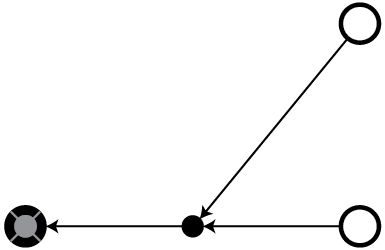
\includegraphics[width=\textwidth]{./img/method_experiment_merging}
		%!TEX root = ../report.tex

\begin{tikzpicture}
	\node[source, label={left:(100, 50)}, state, initial, initial text={}, initial where=above]			
		(c_0)						{$\mathbf{s_0}$};
	\node[source, label=below:{(100, -50)}, state, initial, initial text={}, initial where=right]		
		(c_1)	[below of=c_0] 		{$\mathbf{s_1}$};
	\node[vertex, label=below:{(0, -50)}, state]														
		(v_0) 	[left of=c_1]    	{$v_0$};
	\node[sink, label=below:{(-100, -50)}, state, accepting]										
		(k_0) 	[left of=v_0]		{$\mathbf{s_2}$};

	\path[->] (c_0) edge[edgeStyle] (v_0);
	\path[->] (v_0) edge[edgeStyle] (k_0);
	\path[->] (c_1) edge[edgeStyle] (v_0);
\end{tikzpicture}
		\caption{Merging traffic}
		\label{fig:method:experiment:merging}
	\end{subfigure}
	\begin{subfigure}{0.49\textwidth}
		\centering
		% 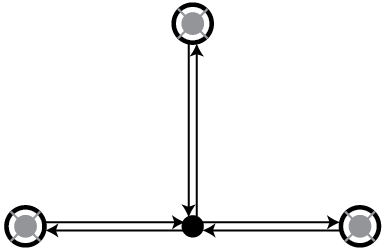
\includegraphics[width=\textwidth]{./img/method_experiment_intersection}
		%!TEX root = ../report.tex

\begin{tikzpicture}

	\node[label=left:{(0, 10)}, state, initial, initial text={}, initial where=above, accepting, source, sink]		
		(s_0)						{$s_0$};
	\node[vertex, label=below:{(0, -10)}, state]														
		(v_0) 	[below of=s_0]    	{$v_0$};
	\node[label=below:{(10, -10)}, state, initial, initial text={}, initial where=right, accepting, source, sink]		
		(s_1)	[right of=v_0] 		{$s_1$};
	\node[label=below:{(-10, -10)}, state, initial, initial text={}, initial where=left, accepting, source, sink]	
		(s_2)	[left of=v_0] 		{$s_2$};

	\path[->] (s_0) edge[edgeStyle] (v_0);
	\path[->] (v_0) edge[edgeStyle] (s_0);

	\path[->] (s_1) edge[edgeStyle] (v_0);
	\path[->] (v_0) edge[edgeStyle] (s_1);	

	\path[->] (s_2) edge[edgeStyle] (v_0);
	\path[->] (v_0) edge[edgeStyle] (s_2);		
\end{tikzpicture}
		\caption{Intersecting traffic}
		\label{fig:method:experiment:intersection}
	\end{subfigure}	
	% \caption{The graphs representing the network of streets used in our experiment, \subref{fig:method:experiment:merging} shows a graph that forces traffic to merge into a different lane with traffic, \subref{fig:method:experiment:intersection} presents a graph that forces cars to cross other traffic. In these graphs solid black circles indicate `normal' vertices, white circles with a black border are sources and the grey crossed out circles denote sinks.}
	\caption{The graphs representing the network of streets used in our experiment, \subref{fig:method:experiment:merging} shows a graph that forces traffic to merge into a different lane with traffic, \subref{fig:method:experiment:intersection} presents a graph that forces cars to cross other traffic. In these graphs filled vertices with a double border indicate sinks. A thick arrow indicates sources, which have a red border. Associated with each node is a location in the simulation space and a name.}
	\label{fig:method:experimentGraphs}
\end{figure}

\subsubsection{Measures}
\label{ss:method:experiment:measures}
\baakman{Wat meten we, hoe heeft dat relatie met RL}
\baakman{Hoe meten we het}

\baakman{Hoe lang laten we het spul lopen enzo.}





% To test if autonomous vehicles have an influence on traffic delays and crashes, we run the simulation multiple times, with different autonomous vehicle to human driver ratios.

% For each of these runs, we measure the time it takes for each agent to reach its goal, relative to the distance they have to travel from their initial position to the target. Furthermore we keep track of the number of collisions with other agents. 

% Using these measurements, we  determine if the number of collisions and the delay time are influenced by the ratio of autonomous agents to the human ones. 

% \baakman{Welke statistieken hebben we? Hoe rekenen we ze uit? Waarom zijn ze relevant.}

% \baakman{Welke twee grafen (Invoegen, T-splitsing) gebruiken we, waarom deze, plaatjes enzo.}

% \baakman{Hoe vaak runnen we, met welke initiele parameters runnen we. Hoe lang runnen we.}